\documentclass{beamer}
\usepackage[latin1]{inputenc}
%\usetheme{Montpellier}
%\usetheme{Boadilla}
%\usecolortheme[RGB={204,51,255}]{structure}
%\usecolortheme[named=purple]{structure}
\usecolortheme[RGB={128,62,62}]{structure}
%\definecolor{dark}{rgb}{0.3,0.15,0.3}
%\definecolor{light}{rgb}{0.8,0.6,0.8}
%\definecolor{reddish}{rgb}{.5,0.15,0.15}
\definecolor{dark}{rgb}{0.5,0.3,0.4}
%\definecolor{light}{rgb}{0.8,0.6,0.8}
\definecolor{reddish}{rgb}{.7,0.25,0.25}
\definecolor{greenish}{rgb}{.25,0.7,0.25}
\definecolor{blueish}{rgb}{.25,0.25,0.7}
\definecolor{purple}{rgb}{.5,0.0,0.5}
\usepackage{graphicx}
\usepackage{pstricks}

\usepackage{amssymb}

\usepackage{amsmath}
\setbeamertemplate{navigation symbols}{}

\newcommand{\crish}{\color{reddish}}
\newcommand{\cbla}{\color{black}}
\newcommand{\cred}{\color{red}}
\newcommand{\cblu}{\color{blue}}
\newcommand{\cgre}{\color{green}}

\newcommand{\sm}{\color{reddish}$}
\newcommand{\fm}{$\color{black}}
\usepackage{tikz}
\usetikzlibrary{arrows,decorations.markings,positioning}
\usetikzlibrary{calc,fit,shapes, backgrounds} 

\usepackage{epstopdf}
\title{Lecture 15: Continuous distributions}
\author{COMS10014 Mathematics for Computer Science A}
\institute{\texttt{cs-uob.github.io/COMS10014/ and github.com/coms10011/2020\_21}}
\date{December 2020}
\begin{document}

\maketitle

\begin{frame}{Finding an average sized baby}
  \begin{center}
    \includegraphics[width=10cm]{baby_weigh.jpg}
  \end{center}
\end{frame}


\begin{frame}{Finding an average sized baby}
  \begin{center}
    \includegraphics[width=10cm]{baby_scale.jpg}
  \end{center}
\end{frame}

\begin{frame}{Probabilities}

  We don't mean `what is the probability of a baby weighing 2.75kg',
  we mean, what is the probability of a baby in a small range around 2.75kg:
  \crish$$P(W\in [2.745,2.755])$$\cbla{}

\end{frame}

\begin{frame}{Cumulative and density}

  We describe the probability distribution with a \textbf{distribution function} or \textbf{cumulative}:
\crish$$F(x)=P(X<x)$$\cbla{}
or a \textbf{density function}:
\crish$$f(x)=\frac{dF}{dx}$$\cbla{}
with
\crish$$
F(x)=\int_{-\infty}^x f(y)dy
$$\cbla{}
\end{frame}

\begin{frame}{Cumulative and density}
\crish$$F(x)=P(X<x)$$\cbla{}
with
\crish$$
F(x)=\int_{-\infty}^x f(y)dy
$$\cbla{}
so
\crish$$
\lim_{x\rightarrow \infty}F(x)=1
$$\cbla{}
or
\crish$$
\int_{-\infty}^\infty f(y)dy=1
$$\cbla{}
\end{frame}

\begin{frame}{Probabilities}
\crish$$
P(x\in [x_1,x_2])=P(x\le x_2)-P(x<x_1)
$$\cbla{}
For a continuous variable we don't have to be careful about the
distinction between \crish$x<x_2$\cbla{}  and \crish$x\le x_2$\cbla{}. Hence
\crish$$
P(x\in [x_1,x_2])=F(x_2)-F(x_1)
$$\cbla{}
or
\crish$$
P(x\in [x_1,x_2])=\int_{x_1}^{x_2} f(y)dy
$$\cbla{}
\end{frame}

\begin{frame}{Constant density}
\crish$$
f(x)=\left\{\begin{array}{ll}\frac{1}{2}&x\in [-1,1]\\0&\mbox{otherwise}\end{array}\right.
$$\cbla{}
\begin{center}
% GNUPLOT: LaTeX picture with Postscript
\begingroup
  \makeatletter
  \providecommand\color[2][]{%
    \GenericError{(gnuplot) \space\space\space\@spaces}{%
      Package color not loaded in conjunction with
      terminal option `colourtext'%
    }{See the gnuplot documentation for explanation.%
    }{Either use 'blacktext' in gnuplot or load the package
      color.sty in LaTeX.}%
    \renewcommand\color[2][]{}%
  }%
  \providecommand\includegraphics[2][]{%
    \GenericError{(gnuplot) \space\space\space\@spaces}{%
      Package graphicx or graphics not loaded%
    }{See the gnuplot documentation for explanation.%
    }{The gnuplot epslatex terminal needs graphicx.sty or graphics.sty.}%
    \renewcommand\includegraphics[2][]{}%
  }%
  \providecommand\rotatebox[2]{#2}%
  \@ifundefined{ifGPcolor}{%
    \newif\ifGPcolor
    \GPcolorfalse
  }{}%
  \@ifundefined{ifGPblacktext}{%
    \newif\ifGPblacktext
    \GPblacktexttrue
  }{}%
  % define a \g@addto@macro without @ in the name:
  \let\gplgaddtomacro\g@addto@macro
  % define empty templates for all commands taking text:
  \gdef\gplbacktext{}%
  \gdef\gplfronttext{}%
  \makeatother
  \ifGPblacktext
    % no textcolor at all
    \def\colorrgb#1{}%
    \def\colorgray#1{}%
  \else
    % gray or color?
    \ifGPcolor
      \def\colorrgb#1{\color[rgb]{#1}}%
      \def\colorgray#1{\color[gray]{#1}}%
      \expandafter\def\csname LTw\endcsname{\color{white}}%
      \expandafter\def\csname LTb\endcsname{\color{black}}%
      \expandafter\def\csname LTa\endcsname{\color{black}}%
      \expandafter\def\csname LT0\endcsname{\color[rgb]{1,0,0}}%
      \expandafter\def\csname LT1\endcsname{\color[rgb]{0,1,0}}%
      \expandafter\def\csname LT2\endcsname{\color[rgb]{0,0,1}}%
      \expandafter\def\csname LT3\endcsname{\color[rgb]{1,0,1}}%
      \expandafter\def\csname LT4\endcsname{\color[rgb]{0,1,1}}%
      \expandafter\def\csname LT5\endcsname{\color[rgb]{1,1,0}}%
      \expandafter\def\csname LT6\endcsname{\color[rgb]{0,0,0}}%
      \expandafter\def\csname LT7\endcsname{\color[rgb]{1,0.3,0}}%
      \expandafter\def\csname LT8\endcsname{\color[rgb]{0.5,0.5,0.5}}%
    \else
      % gray
      \def\colorrgb#1{\color{black}}%
      \def\colorgray#1{\color[gray]{#1}}%
      \expandafter\def\csname LTw\endcsname{\color{white}}%
      \expandafter\def\csname LTb\endcsname{\color{black}}%
      \expandafter\def\csname LTa\endcsname{\color{black}}%
      \expandafter\def\csname LT0\endcsname{\color{black}}%
      \expandafter\def\csname LT1\endcsname{\color{black}}%
      \expandafter\def\csname LT2\endcsname{\color{black}}%
      \expandafter\def\csname LT3\endcsname{\color{black}}%
      \expandafter\def\csname LT4\endcsname{\color{black}}%
      \expandafter\def\csname LT5\endcsname{\color{black}}%
      \expandafter\def\csname LT6\endcsname{\color{black}}%
      \expandafter\def\csname LT7\endcsname{\color{black}}%
      \expandafter\def\csname LT8\endcsname{\color{black}}%
    \fi
  \fi
  \setlength{\unitlength}{0.0500bp}%
  \begin{picture}(3600.00,2520.00)%
    \gplgaddtomacro\gplbacktext{%
      \csname LTb\endcsname%
      \put(726,743){\makebox(0,0)[r]{\strut{} 0}}%
      \put(726,1348){\makebox(0,0)[r]{\strut{} 0.5}}%
      \put(726,1953){\makebox(0,0)[r]{\strut{} 1}}%
      \put(858,220){\makebox(0,0){\strut{}-2}}%
      \put(1444,220){\makebox(0,0){\strut{}-1}}%
      \put(2031,220){\makebox(0,0){\strut{} 0}}%
      \put(2617,220){\makebox(0,0){\strut{} 1}}%
      \put(3203,220){\makebox(0,0){\strut{} 2}}%
    }%
    \gplgaddtomacro\gplfronttext{%
    }%
    \gplbacktext
    \put(0,0){
\includegraphics{fig_p_const}}%
    \gplfronttext
  \end{picture}%
\endgroup

\end{center}

\end{frame}


\begin{frame}{Constant density}
\crish$$
F(x)=\left\{\begin{array}{ll}0&x<-1\\
\frac{x+1}{2}&x\in [-1,1]\\1&x>1\end{array}\right.
$$\cbla{}

\begin{center}
% GNUPLOT: LaTeX picture with Postscript
\begingroup
  \makeatletter
  \providecommand\color[2][]{%
    \GenericError{(gnuplot) \space\space\space\@spaces}{%
      Package color not loaded in conjunction with
      terminal option `colourtext'%
    }{See the gnuplot documentation for explanation.%
    }{Either use 'blacktext' in gnuplot or load the package
      color.sty in LaTeX.}%
    \renewcommand\color[2][]{}%
  }%
  \providecommand\includegraphics[2][]{%
    \GenericError{(gnuplot) \space\space\space\@spaces}{%
      Package graphicx or graphics not loaded%
    }{See the gnuplot documentation for explanation.%
    }{The gnuplot epslatex terminal needs graphicx.sty or graphics.sty.}%
    \renewcommand\includegraphics[2][]{}%
  }%
  \providecommand\rotatebox[2]{#2}%
  \@ifundefined{ifGPcolor}{%
    \newif\ifGPcolor
    \GPcolorfalse
  }{}%
  \@ifundefined{ifGPblacktext}{%
    \newif\ifGPblacktext
    \GPblacktexttrue
  }{}%
  % define a \g@addto@macro without @ in the name:
  \let\gplgaddtomacro\g@addto@macro
  % define empty templates for all commands taking text:
  \gdef\gplbacktext{}%
  \gdef\gplfronttext{}%
  \makeatother
  \ifGPblacktext
    % no textcolor at all
    \def\colorrgb#1{}%
    \def\colorgray#1{}%
  \else
    % gray or color?
    \ifGPcolor
      \def\colorrgb#1{\color[rgb]{#1}}%
      \def\colorgray#1{\color[gray]{#1}}%
      \expandafter\def\csname LTw\endcsname{\color{white}}%
      \expandafter\def\csname LTb\endcsname{\color{black}}%
      \expandafter\def\csname LTa\endcsname{\color{black}}%
      \expandafter\def\csname LT0\endcsname{\color[rgb]{1,0,0}}%
      \expandafter\def\csname LT1\endcsname{\color[rgb]{0,1,0}}%
      \expandafter\def\csname LT2\endcsname{\color[rgb]{0,0,1}}%
      \expandafter\def\csname LT3\endcsname{\color[rgb]{1,0,1}}%
      \expandafter\def\csname LT4\endcsname{\color[rgb]{0,1,1}}%
      \expandafter\def\csname LT5\endcsname{\color[rgb]{1,1,0}}%
      \expandafter\def\csname LT6\endcsname{\color[rgb]{0,0,0}}%
      \expandafter\def\csname LT7\endcsname{\color[rgb]{1,0.3,0}}%
      \expandafter\def\csname LT8\endcsname{\color[rgb]{0.5,0.5,0.5}}%
    \else
      % gray
      \def\colorrgb#1{\color{black}}%
      \def\colorgray#1{\color[gray]{#1}}%
      \expandafter\def\csname LTw\endcsname{\color{white}}%
      \expandafter\def\csname LTb\endcsname{\color{black}}%
      \expandafter\def\csname LTa\endcsname{\color{black}}%
      \expandafter\def\csname LT0\endcsname{\color{black}}%
      \expandafter\def\csname LT1\endcsname{\color{black}}%
      \expandafter\def\csname LT2\endcsname{\color{black}}%
      \expandafter\def\csname LT3\endcsname{\color{black}}%
      \expandafter\def\csname LT4\endcsname{\color{black}}%
      \expandafter\def\csname LT5\endcsname{\color{black}}%
      \expandafter\def\csname LT6\endcsname{\color{black}}%
      \expandafter\def\csname LT7\endcsname{\color{black}}%
      \expandafter\def\csname LT8\endcsname{\color{black}}%
    \fi
  \fi
  \setlength{\unitlength}{0.0500bp}%
  \begin{picture}(3600.00,2520.00)%
    \gplgaddtomacro\gplbacktext{%
      \csname LTb\endcsname%
      \put(726,743){\makebox(0,0)[r]{\strut{} 0}}%
      \put(726,1348){\makebox(0,0)[r]{\strut{} 0.5}}%
      \put(726,1953){\makebox(0,0)[r]{\strut{} 1}}%
      \put(858,220){\makebox(0,0){\strut{}-2}}%
      \put(1444,220){\makebox(0,0){\strut{}-1}}%
      \put(2031,220){\makebox(0,0){\strut{} 0}}%
      \put(2617,220){\makebox(0,0){\strut{} 1}}%
      \put(3203,220){\makebox(0,0){\strut{} 2}}%
    }%
    \gplgaddtomacro\gplfronttext{%
    }%
    \gplbacktext
    \put(0,0){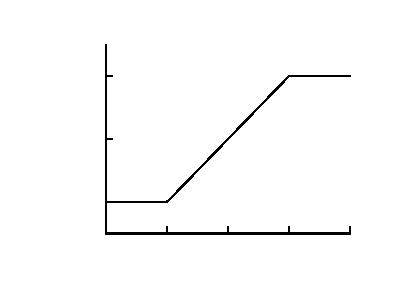
\includegraphics{fig_c_const}}%
    \gplfronttext
  \end{picture}%
\endgroup

\end{center}

\end{frame}

\begin{frame}{Properties}
  \crish$F(x)\ge F(y)$\cbla{} if \crish$x>y$\cbla{} so it is monotonically increasing function so
  \crish$$p(x)=\frac{dF(x)}{dx}\ge 0$$\cbla{}
\end{frame}

\begin{frame}{Properties}
  Clearly
\crish$$
  P(x\in [a,b])=\int_a^bf(y)dy\le 1
$$\cbla{}
  but \crish$p(x)$\cbla{} can be greater than one. For example
\crish$$
f(x)=\left\{\begin{array}{ll}4&x\in [0,1/4]\\0&\mbox{otherwise}\end{array}\right.
$$\cbla{}
\end{frame}
  

\begin{frame}{Properties}
\crish$$
f(x)=\left\{\begin{array}{ll}4&x\in [0,1/4]\\0&\mbox{otherwise}\end{array}\right.
$$\cbla{}

\begin{center}
% GNUPLOT: LaTeX picture with Postscript
\begingroup
  \makeatletter
  \providecommand\color[2][]{%
    \GenericError{(gnuplot) \space\space\space\@spaces}{%
      Package color not loaded in conjunction with
      terminal option `colourtext'%
    }{See the gnuplot documentation for explanation.%
    }{Either use 'blacktext' in gnuplot or load the package
      color.sty in LaTeX.}%
    \renewcommand\color[2][]{}%
  }%
  \providecommand\includegraphics[2][]{%
    \GenericError{(gnuplot) \space\space\space\@spaces}{%
      Package graphicx or graphics not loaded%
    }{See the gnuplot documentation for explanation.%
    }{The gnuplot epslatex terminal needs graphicx.sty or graphics.sty.}%
    \renewcommand\includegraphics[2][]{}%
  }%
  \providecommand\rotatebox[2]{#2}%
  \@ifundefined{ifGPcolor}{%
    \newif\ifGPcolor
    \GPcolorfalse
  }{}%
  \@ifundefined{ifGPblacktext}{%
    \newif\ifGPblacktext
    \GPblacktexttrue
  }{}%
  % define a \g@addto@macro without @ in the name:
  \let\gplgaddtomacro\g@addto@macro
  % define empty templates for all commands taking text:
  \gdef\gplbacktext{}%
  \gdef\gplfronttext{}%
  \makeatother
  \ifGPblacktext
    % no textcolor at all
    \def\colorrgb#1{}%
    \def\colorgray#1{}%
  \else
    % gray or color?
    \ifGPcolor
      \def\colorrgb#1{\color[rgb]{#1}}%
      \def\colorgray#1{\color[gray]{#1}}%
      \expandafter\def\csname LTw\endcsname{\color{white}}%
      \expandafter\def\csname LTb\endcsname{\color{black}}%
      \expandafter\def\csname LTa\endcsname{\color{black}}%
      \expandafter\def\csname LT0\endcsname{\color[rgb]{1,0,0}}%
      \expandafter\def\csname LT1\endcsname{\color[rgb]{0,1,0}}%
      \expandafter\def\csname LT2\endcsname{\color[rgb]{0,0,1}}%
      \expandafter\def\csname LT3\endcsname{\color[rgb]{1,0,1}}%
      \expandafter\def\csname LT4\endcsname{\color[rgb]{0,1,1}}%
      \expandafter\def\csname LT5\endcsname{\color[rgb]{1,1,0}}%
      \expandafter\def\csname LT6\endcsname{\color[rgb]{0,0,0}}%
      \expandafter\def\csname LT7\endcsname{\color[rgb]{1,0.3,0}}%
      \expandafter\def\csname LT8\endcsname{\color[rgb]{0.5,0.5,0.5}}%
    \else
      % gray
      \def\colorrgb#1{\color{black}}%
      \def\colorgray#1{\color[gray]{#1}}%
      \expandafter\def\csname LTw\endcsname{\color{white}}%
      \expandafter\def\csname LTb\endcsname{\color{black}}%
      \expandafter\def\csname LTa\endcsname{\color{black}}%
      \expandafter\def\csname LT0\endcsname{\color{black}}%
      \expandafter\def\csname LT1\endcsname{\color{black}}%
      \expandafter\def\csname LT2\endcsname{\color{black}}%
      \expandafter\def\csname LT3\endcsname{\color{black}}%
      \expandafter\def\csname LT4\endcsname{\color{black}}%
      \expandafter\def\csname LT5\endcsname{\color{black}}%
      \expandafter\def\csname LT6\endcsname{\color{black}}%
      \expandafter\def\csname LT7\endcsname{\color{black}}%
      \expandafter\def\csname LT8\endcsname{\color{black}}%
    \fi
  \fi
    \setlength{\unitlength}{0.0500bp}%
    \ifx\gptboxheight\undefined%
      \newlength{\gptboxheight}%
      \newlength{\gptboxwidth}%
      \newsavebox{\gptboxtext}%
    \fi%
    \setlength{\fboxrule}{0.5pt}%
    \setlength{\fboxsep}{1pt}%
\begin{picture}(3600.00,2520.00)%
    \gplgaddtomacro\gplbacktext{%
      \csname LTb\endcsname%%
      \put(330,647){\makebox(0,0)[r]{\strut{}$0$}}%
      \put(330,1473){\makebox(0,0)[r]{\strut{}$2$}}%
      \put(330,2300){\makebox(0,0)[r]{\strut{}$4$}}%
      \put(462,220){\makebox(0,0){\strut{}$-1$}}%
      \put(1147,220){\makebox(0,0){\strut{}$-0.5$}}%
      \put(1833,220){\makebox(0,0){\strut{}$0$}}%
      \put(2518,220){\makebox(0,0){\strut{}$0.5$}}%
      \put(3203,220){\makebox(0,0){\strut{}$1$}}%
    }%
    \gplgaddtomacro\gplfronttext{%
    }%
    \gplbacktext
    \put(0,0){
\includegraphics{narrow}}%
    \gplfronttext
  \end{picture}%
\endgroup

\end{center}

\end{frame}




\end{document}

